\documentclass{article}
\usepackage[UTF8]{ctex}
\usepackage{amsmath,amssymb}
\usepackage{geometry}
\usepackage{graphicx}
\geometry{left=2.5cm,right=2.5cm,top=2.5cm,bottom=3cm}
\numberwithin{equation}{section}
\title{计算物理学第一次作业}
\begin{document}
\maketitle
\section{数值误差的避免}
\subsection*{(a)}
根据题意,我们令
\begin{align}
    \epsilon=\frac{\epsilon_M}{2}
\end{align}
按照计算机的求和顺序,可以得到
\begin{align}
    \overline{x}          & =  \frac{1}{N} \sum_{i=1}^N x_i                                                                                                 \\
    \overline{x}^{\prime} & =  \frac{1}{N} \left(\left(x_1\left(1+\epsilon\right)+x_2\right)\left(1+\epsilon\right)\cdots+x_N\right)\left(1+\epsilon\right) \\
                          & =  \frac{1}{N} \left[\sum_{i=1}^N x_i+\sum_{i=1}^N x_i\left(N+1-i\right)\epsilon\right]
\end{align}
若要估计舍入误差的最大上限,可以设
\begin{align}
    \begin{cases}
        x_i=x_1 & i=1,          \\
        x_i=0   & i=2,3\cdots N
    \end{cases}
\end{align}
则最后得到
\begin{align}
    \overline{x}^{\prime}                                   & =\frac{x_1}{N}+\frac{x_1N\epsilon}{N} \\
                                                            & =\overline{x}+\overline{x}N\epsilon   \\
    \frac{\overline{x}^{\prime}-\overline{x}}{\overline{x}} & = N\epsilon=N\frac{\epsilon_M}{2}
\end{align}
\subsection*{(b)}
显然,上式中出现大数相减,下式先平方在求和,因此是下式更稳定。
\subsection*{(c)}
\begin{align}
    I_0=\int_0^1 \frac{1}{x+5}\mathrm{d}x=\ln \frac{6}{5}
\end{align}
\begin{align}
    I_k+5I_{k-1} & =\int_0^1 \frac{x^k+5x^{k-1}}{x+5}\mathrm{d}x \\
                 & =\int_0^1 x^{k-1}\mathrm{d}x                  \\
                 & =\frac{1}{k}
\end{align}
如果计算时出现微小误差使得
\begin{align}
    I_0^{\prime}=I_0\left(1+\epsilon\right)
\end{align}
则最后得到
\begin{align}
    I_n=\left(-5\right)^n I_0 \epsilon
\end{align}
显然不是稳定的
\section{矩阵的模与条件数}
\subsection*{(a)}
\begin{align}
    \det\left(A\right)=\prod_{i=1}^n 1=1 \neq 0
\end{align}
因此是非奇异矩阵。
\subsection*{(b)}
\begin{align}
    A^{-1}=\begin{pmatrix}
        1 & 1 & 2 & 4 & \cdots & 2^{n-2} \\
        0 & 1 & 1 & 2 & \ddots & \vdots  \\
        0 & 0 & 1 & 1 & 2      & 4       \\
        0 & 0 & 0 & 1 & 1      & 2       \\
        0 & 0 & 0 & 0 & 1      & 1       \\
        0 & 0 & 0 & 0 & 0      & 1
    \end{pmatrix}
\end{align}
\subsection*{(c)}
做一个不影响最终结果的假设:
\begin{align}
    \max_{i=1,\cdots,n}\left| x_i \right|=1
\end{align}
因此
\begin{align}
          & \frac{\max_{i=1,\cdots,n}\left|\sum_{j=1}^n a_{ij}x_j\right|}{\max_{i=1,\cdots,n}\left|x_i\right|} \\
    =     & \max_{i=1,\cdots,n}\left|\sum_{j=1}^n a_{ij}x_j\right|                                             \\
    \leqq & \max_{i=1,\cdots,n}\sum_{j=1}^n \left|a_{ij}\right|\left|x_j\right|                                \\
    \leqq & \max_{i=1,\cdots,n}\sum_{j=1}^n \left|a_{ij}\right|
\end{align}
当$\left| x_i \right|=1$时,等号成立。证毕
\subsection*{(d)}
\begin{align}
    \Vert U\Vert_2 & =\frac{\left(\left(Ux\right)^*Ux\right)^{\frac{1}{2}}}{\left(x^*x\right)^{\frac{1}{2}}} \\
                   & =\frac{\left(x^*U^*Ux\right)^{\frac{1}{2}}}{\left(x^*x\right)^{\frac{1}{2}}}            \\
                   & =1
\end{align}
同理
\begin{align}
    \Vert U\Vert_2=\Vert U^\dagger\Vert_2=1
\end{align}
\begin{align}
    \Vert UA\Vert_2 & =\frac{\left(\left(UAx\right)^*UAx\right)^{\frac{1}{2}}}{\left(x^*x\right)^{\frac{1}{2}}} \\
                    & =\frac{\left(x^*A^*U^*UAx\right)^{\frac{1}{2}}}{\left(x^*x\right)^{\frac{1}{2}}}          \\
                    & =\frac{\left(x^*A^*Ax\right)^{\frac{1}{2}}}{\left(x^*x\right)^{\frac{1}{2}}}              \\
                    & =\Vert A\Vert_2
\end{align}
\subsection*{(e)}
\begin{align}
    \Vert A\Vert_\infty      & =1                                                   \\
    \Vert A^{-1}\Vert_\infty & =2^{n-2}                                             \\
    K_\infty\left(A\right)   & =\Vert A\Vert_\infty\Vert A^{-1}\Vert_\infty=2^{n-2}
\end{align}
\section{Hilbert矩阵}
\subsection*{(a)}
\begin{align}
    D=\int_0^1 \mathrm{d}x \left(\sum_{j=1}^n c_j x^{j-1}-f\left(x\right)\right)^2
\end{align}
取极值,则有
\begin{gather}
    \frac{\partial D}{\partial c_i}=0                                                         \\
    \int_0^1 \left(\sum_{j=1}^n c_j x^{j-1}-f\left(x\right)\right)x^{j-1}\mathrm{d}x=0        \\
    \sum_{j=1}^n \int_0^1 c_j x^{i+j-2}\mathrm{d}x=\int_0^1 f\left(x\right)x^{i-1}\mathrm{d}x \\
    \sum_{j=1}^n \frac{c_j}{i+j-1}=\int_0^1 f\left(x\right)x^{j-1}\mathrm{d}x
\end{gather}
故
\begin{align}
    \begin{cases}
        \left(H_{n}\right)_{ij}=\frac{1}{i+j-1} \\
        b_i=\int_0^1 f\left(x\right)x^{i-1}\mathrm{d}x
    \end{cases}
\end{align}
\subsection*{(b)}
由于$\left(H_{n}\right)_{ij}=\frac{1}{i+j-1}$,对称性是显然的。
\begin{align}
      & \int_0^1 \left(\sum_{i=0}^n c_i x^{i-1}\right)^2\mathrm{d}x                \\
    = & \int_0^1 \sum_{i=0}^n c_i x^{i-1}\cdot \sum_{j=0}^n c_j x^{j-1}\mathrm{d}x \\
    = & \int_0^1 \sum_{i=0}^n \sum_{j=0}^n c_i c_j x^{i+j-2}\mathrm{d}x            \\
    = & \sum_{i=0}^n \sum_{j=0}^n \frac{c_i c_j}{i+j-1}                            \\
    = & c^{\mathrm{T}}H_nc
\end{align}
由于被积函数大于等于0,因此$c^{\mathrm{T}}H_nc\geqq 0$。\\
显然当且仅当$\sum_{i=0}^n c_i x^{i-1}\equiv 0$,即$c_i=0$时成立。\par
对称实矩阵的所有本征值为实数。由于$H_n$为对称正定实矩阵,因此其本征值均大于0。故
\begin{align}
    \det\left(H_n\right)=\prod_{i=1}^s \lambda^{r_i}\geq 0
\end{align}
即$H_n$是非奇异的
\subsection*{(c)}
\begin{align}
    \frac{1}{\det\left(H_n\right)}=n!\cdot\sum_{i=1}^{2n-1}\begin{pmatrix}
        i \\
        \left[\frac{i}{2}\right]
    \end{pmatrix} \\
\end{align}
代入斯特灵公式得到
\begin{align}
    \det\left(H_n\right)=0.645x^{-1/4} (2\pi)^x 4^{-x^2}
\end{align}
\subsection*{(d)}
经解得,高斯消元法更精确。如图,也可以运行 3(d).py 查看结果。\\
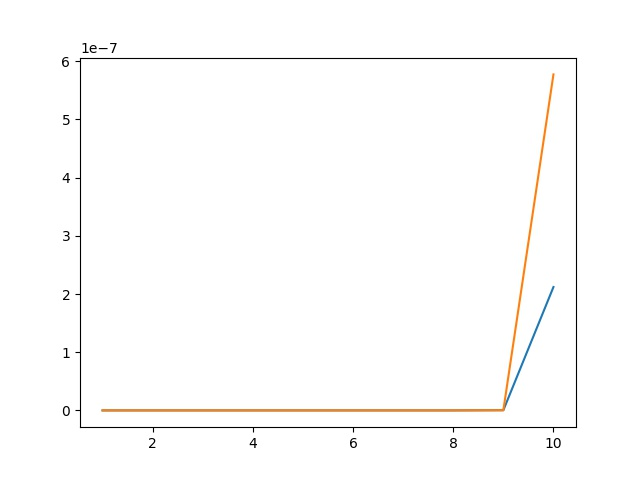
\includegraphics[scale=0.4]{assets/3(d).jpg}
\section{级数求和与截断误差}
\subsection*{(a)}
第三小问给出了详细求解过程
\begin{align}
    f\left(q^2\right)_{q^2=0.5}=1.10622
\end{align}
\subsection*{(b)}
将这个求和减积分的式子拆分成从$n\in \left[0,1\right)$,$n\in \left[1,2\right)$...$n\in \left[R,R+1\right)$\\
利用程序求出
\begin{align}
    g\left(R\right)=\underset{\left|\vec{n}\right|\in\left[R,R+1\right)}{\left(\sum-\mathcal{PV}\int\mathrm{d}^3n\right)}\frac{1}{\left|\vec{n}\right|^2-q^2}
\end{align}
若当$R>>1$且$\overline{g\left(R\right)}<<\left|g\left(R\right)\right|<10^{-5}$,则可以认为精度达到了$10^{-5}$。\\
\\
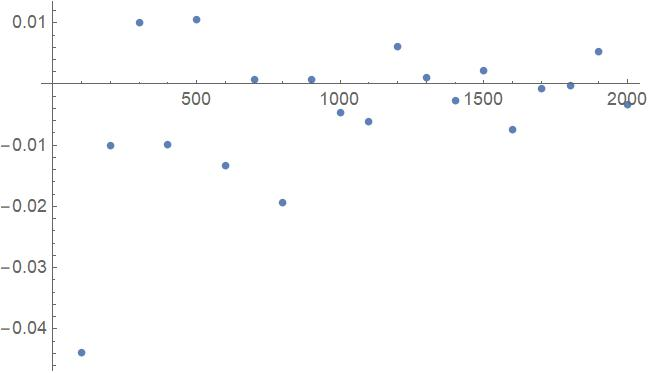
\includegraphics[scale=0.4]{assets/4(c)1.jpg}
\\
可以看到即便当$R=2000$时,误差依旧较大。且收敛较慢不便外推。\\
在此做一个假设,即误差主要受求和项中$n^2=R^2$的影响,因为当$R$截止于不同位置,即$R+$或$R-$处,将会造成一个突变。突变项即为当$n^2=R^2$时求和项的值。\\
求出该项的值并作图 见 4.cpp\\
\\
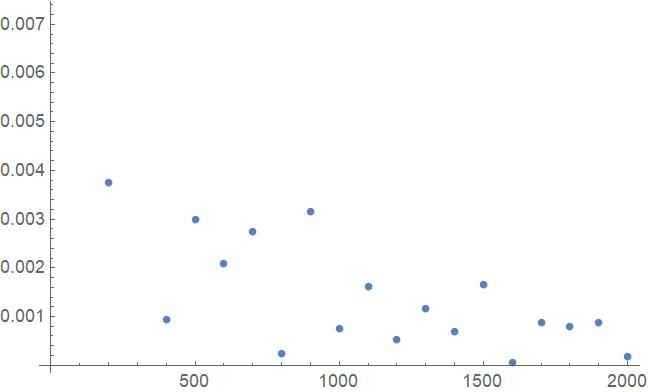
\includegraphics[scale=0.4]{assets/4(c)2.jpg}\\
\\
可以看到误差与$1/R$为同一量级。保守估计,当$\Lambda\sim 10^-6$,此时精度能到达$10^{-5}$
\subsection*{(c)}
为了使求和与积分结果分别能收敛,将式子改写为
\begin{align}
    f\left(q^2,\vec{r}\right)=\sum_{\vec{n} \in \mathbb{Z}^{3}} \frac{e^{i \vec{n} \cdot \vec{r}}}{|\vec{n}|^{2}-q^{2}}-\text{P.V.} \int \mathrm{d}^{3} \vec{n} \frac{e^{i \vec{n} \cdot \vec{r}}}{|\vec{n}|^{2}-q^{2}}
\end{align}
对求和项进行拆分,得到如下两部分
\begin{align}
    \sum_{\vec{n} \in \mathbb{Z}^{3}} \frac{e^{i \vec{n} \cdot \vec{r}}}{|\vec{n}|^{2}-q^{2}} & =\sum_{\vec{n} \in \mathbb{Z}^{3}} \frac{e^{i \vec{n} \cdot \vec{r}} e^{-\left(|\vec{n}|^{2}-q^{2}\right)}}{|\vec{n}|^{2}-q^{2}}+\sum_{\vec{n} \in \mathbb{Z}^{3}} \frac{e^{i \vec{n} \cdot \vec{r}}\left(1-e^{-\left(|\vec{n}|^{2}-q^{2}\right)}\right)}{|\vec{n}|^{2}-q^{2}} \\
                                                                                              & =\sum_{\vec{n} \in \mathbb{Z}^{3}} \frac{e^{i \vec{n} \cdot \vec{r}} e^{-\left(|\vec{n}|^{2}-q^{2}\right)}}{|\vec{n}|^{2}-q^{2}}+\int_{0}^{1} \mathrm{~d} t e^{t q^{2}} \sum_{\vec{n} \in \mathbb{Z}^{3}} e^{i \vec{n} \cdot \vec{r}-t|\vec{n}|^{2}}
\end{align}
对第二部分运用泊松求和公式
\begin{align}
    \sum_{\vec{n} \in \mathbb{Z}^{3}} a(\vec{n})=\sum_{\vec{m} \in \mathbb{Z}^{3}} \hat{a}(\vec{k})
\end{align}
其中$\hat{a}(\vec{k})=\int a(\vec{n}) e^{-2\pi i\vec{k} \cdot \vec{n}}\mathrm{d}^{3}\vec{n} $
代入$a(\vec{n})=e^{i \vec{n} \cdot \vec{r}-t|\vec{n}|^{2}}$,得到
\begin{align}
    \hat{a}(\vec{k}) & =\int \mathrm{d}^{3} \vec{n} e^{i \vec{n} \cdot \vec{r}-t|\vec{n}|^{2}} e^{-2\pi i\vec{k}\cdot\vec{n}}=\int \mathrm{d}^{3} \vec{n} e^{i \vec{n} \cdot(\vec{r}-2\pi\vec{k})-t|\vec{n}|^{2}} \\
                     & =2 \pi \int_{0}^{\infty} \mathrm{d} n n^{2} \int_{0}^{\pi} \mathrm{d}\theta\sin\theta e^{i|\vec{r}-2\pi\vec{k}|n\cos\theta-t n^{2}}                                                        \\
                     & =2 \pi \int_{0}^{\infty} \mathrm{d} n  \frac{2n \sin (n|\vec{r}-2 \pi \vec{k}|)}{|\vec{r}-2 \pi \vec{k}|} e^{-t n^{2}}                                                                     \\
                     & =\left(\frac{\pi}{t}\right)^{3 / 2} e^{-\frac{|r-2 \pi k|^{2}}{4 t}}
\end{align}
可以看到现在的积分内求和收敛的很快。计算出求和项为:
\begin{align}
    \sum_{\vec{n} \in \mathbb{Z}^{3}} \frac{e^{i \vec{n} \cdot \vec{r}}}{|\vec{n}|^{2}-q^{2}} & =\sum_{\vec{n} \in \mathbb{Z}^{3}} \frac{e^{i \vec{n} \cdot \vec{r}} e^{-\left(|\vec{n}|^{2}-q^{2}\right)}}{|\vec{n}|^{2}-q^{2}}+\int_{0}^{1} \mathrm{~d} t e^{t q^{2}} \sum_{\vec{k} \in \mathbb{Z}^{3}}\left(\frac{\pi}{t}\right)^{3 / 2} e^{-\frac{|\tau-2 \pi k|^{2}}{4 t}} \\
                                                                                              & =\sum_{\vec{n} \in \mathbb{Z}^{3}} \frac{e^{i \vec{n} \cdot \vec{r}} e^{-\left(|\vec{n}|^{2}-q^{2}\right)}}{|\vec{n}|^{2}-q^{2}}+\sum_{\vec{k} \in \mathbb{Z}^{3}}\int_{0}^{1} \mathrm{~d} t e^{t q^{2}}\left(\frac{\pi}{t}\right)^{3 / 2} e^{-\frac{|\tau-2 \pi k|^{2}}{4 t}}
\end{align}
当$k=0$且$\vec{r}\to 0$时积分会发散,实际上刚好能与积分项相消。
写出积分项在球坐标中的表达式
\begin{align}
    \text{P.V.} \int \mathrm{d}^{3} \vec{n} \frac{e^{i \vec{n} \cdot \vec{r}}}{\left|\vec{n}\right|^{2}-q^{2}} & =2 \pi \text{P.V.} \int_{0}^{\infty} \mathrm{d} n n^{2} \int_{0}^{\pi} \mathrm{d} \theta \sin \theta \frac{e^{i n r \cos \theta}}{n^{2}-q^{2}} \\
                                                                                                               & =\frac{4 \pi}{r} \text{P.V.} \int_{0}^{\infty} \mathrm{d} n  \frac{n\sin (n r)}{n^{2}-q^{2}}                                                   \\
                                                                                                               & =\frac{2 \pi}{r} \operatorname{Im} \text {P.V.} \int_{-\infty}^{\infty} \mathrm{d} n \frac{n e^{i n r}}{n^{2}-q^{2}}                           \\
                                                                                                               & =\frac{2 \pi^{2}}{r}\cos(qr)
\end{align}
由于最终$\vec{r}\to 0$,可以令
\begin{align}
      & \frac{2 \pi^{2}}{r}\cos(qr)=\frac{2 \pi^{2}}{r}                                                                                 \\
    = & \left.\int_0^\infty \mathrm{d}t \left(\frac{\pi}{t}\right)^{3/2}e^{-\frac{\left|\vec{r}-2\pi k\right|^2}{t}}\right|_{\vec{k}=0}
\end{align}
最后求得
\begin{align}
    f\left(q^2\right)=\sum_{n\in\mathbb{Z}^3} \frac{e^{-\left(\left|\vec{n}\right|^2-q^2\right)}}{\left|\vec{n}\right|^2-q^2}+\int_0^1 \mathrm{d}t e^{tq^2}\sum_{n\in\mathbb{Z}^3\atop n\neq0} \left(\frac{\pi}{t}\right)^{3/2}e^{-\frac{\pi^2\left|\vec{n}\right|^2}{t}}-2\pi^{3/2}e^{q^2}+2\pi^2q\, \mathrm{erfi}\left(q\right)
\end{align}
代入计算机 见 4.py ,得到
\begin{align}
    f\left(q^2\right)=1.10622
\end{align}
\end{document}